\subsection{Quartic Oscillator Results}
\label{sec:qosc_results}

The quartic oscillator \cite{PhysRev.184.1231, girguś2024spiralflowquantumquartic, wójcik2012applicationnumericalrenormalizationgroup} is an extension of the standard harmonic oscillator, modified by an additional non-linearity of the form $\lambda \varphi^4$, leading to the Hamiltonian $H = \frac12\dot\phi^2 + \frac{m}{2}\phi^2 + gm^3\phi^4 $, where $\phi$ represents a bosonic field composed of a single mode.
In a second-quantized, dimensionless form, the Hamiltonian can be written as:

\begin{equation}
    \label{eq:qosc}
    H = a^\dagger a + g\left(a + a^\dagger \right)^4
\end{equation}

It should be obvious that the Hamiltonian written in equation \ref{eq:qosc} is a valid form that can be block-encoded with LOBE, where there is one mode, which can be chosen implicitly to be $0$.
The only `scaling' variable in this problem is the occupancy of the mode $0$, $\Omega$.

\begin{figure}[h]
    \centering
    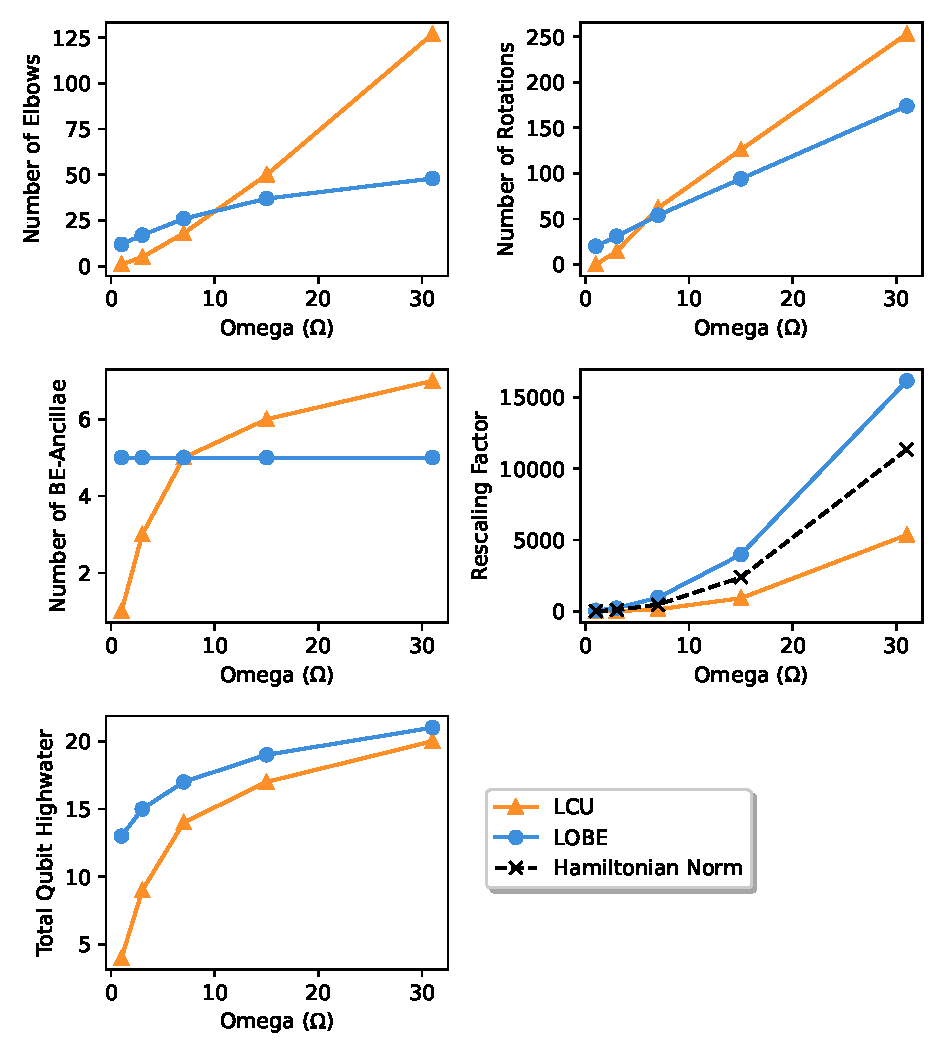
\includegraphics[width = 15cm]{figures/quartic_oscillator.pdf}
    \caption{Costs associated with a single block encoding of the quartic oscillator Hamiltonian \ref{eq:qosc} for LOBE (blue) and LCU (orange).}
    \label{fig:qosc}
\end{figure}
